\section{背景}
\begin{frame}{LD Cycleによる生体リズムの研究}
        \begin{block}{概日リズムの研究:LD Cycle}
          \begin{itemize}
            \item 時差ぼけやシフトワークは、生活習慣病のリスクを高める.
            \item LD Cycleは生体リズムのモデルに用いられ,光と暗闇の情報が外力として系に加わる.\begin{itemize}
              \item 時差ぼけ/シフトワークの研究では,この外力の位相をシフトさせることを考える.
            \end{itemize}
            \item 外力や各パラメータの設定により周期的・カオス的な振る舞いを持つ.
            \item 一般にカオスの予測は難しい(初期値鋭敏性).
          \end{itemize}
        \end{block}
        \vspace{-.5em}
        \begin{figure}
          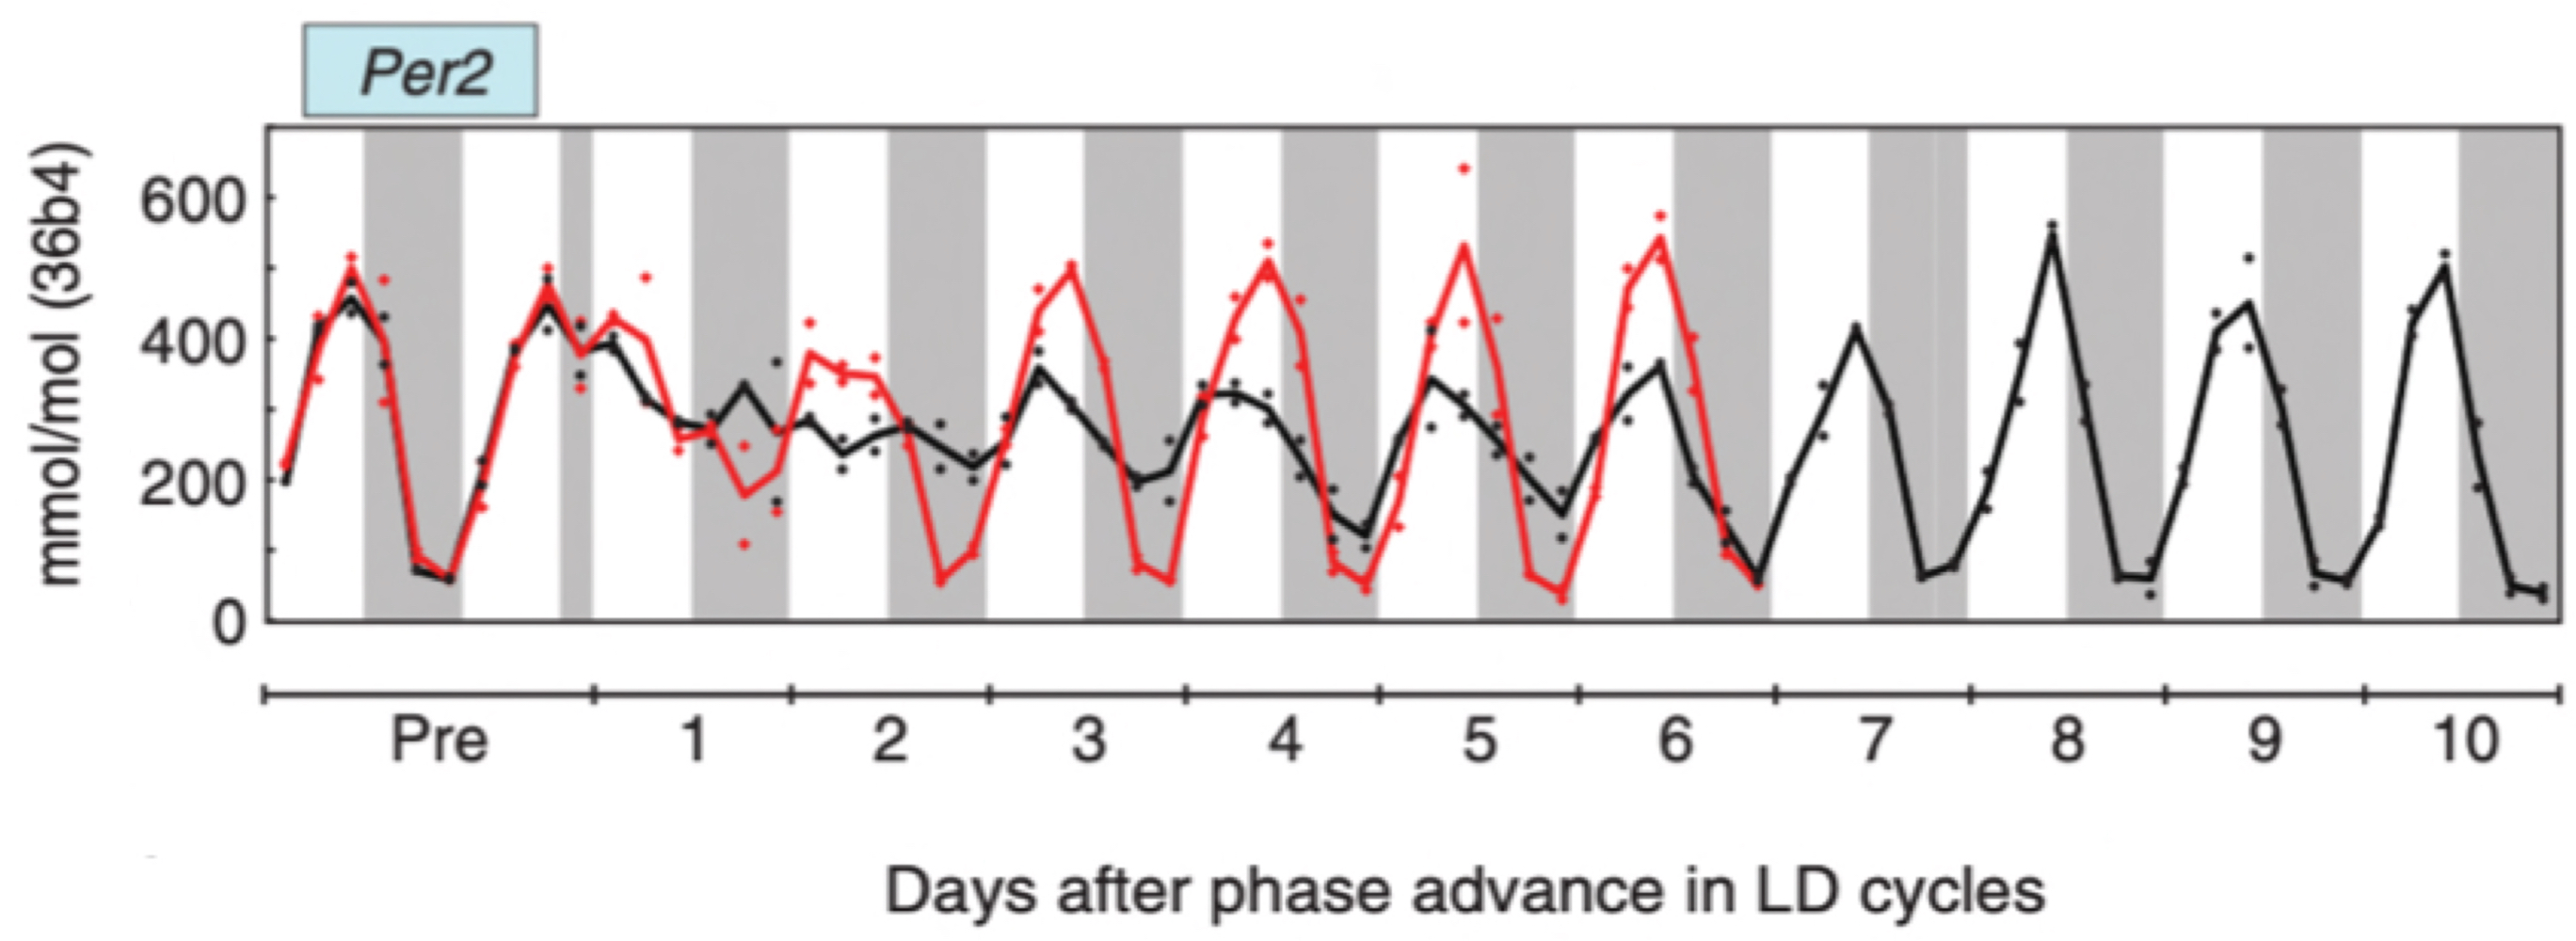
\includegraphics[width=0.4\textwidth]{Fig/Jetlag.png}
          \caption{\scriptsize{Day 1に8時間のJet Lagを受けた時のマウスの Per2 の推移}\\\tiny{Image: Fig.2 from \cite{Yamaguchi et al.}.}}
      \end{figure}    
      
  \end{frame}

  \section{手法}

\begin{frame}{Reservoir Computer の特徴}
    % スライドを2つの列に分割
    \begin{columns}[T] % [T] は列を上部で揃えるオプション
  
      \begin{column}{.5\textwidth}
        
        \begin{itemize}
          \item 右側のアイテム1
          \item 右側のアイテム2
        \end{itemize}
      \end{column}

      \begin{column}{.5\textwidth}
        \begin{figure}
            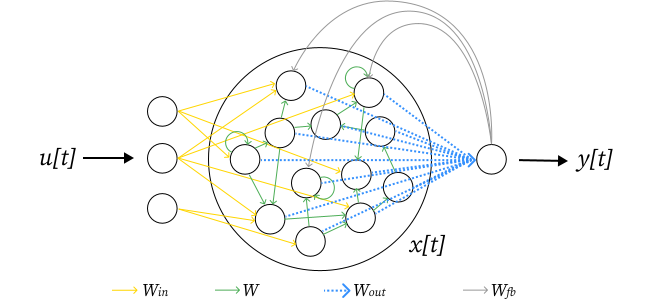
\includegraphics[width=\textwidth]{Fig/esn.svg.png}
        \end{figure}  
        \begin{figure}
            
\includegraphics[width=\textwidth]{Fig/esn_nodes.svg.png}
            \caption{\scriptsize{Reservoirpy での reservoir computer の構造}\\ \tiny{Image: ReservoirPy, MIT License.}}
        \end{figure}  
      \end{column}
    \end{columns}
  \end{frame}


